\chapter{Comunicaci�n entre los componentes}

\textbf{\textit{En este cap�tulo comentamos diferentes implementaciones de la
comunicaci�n entre componentes del sistema. Como veremos, nos centraremos en
los tipos de mensajes en cada tipo de comunicaci�n y la seguridad que debemos
implementar en cada una, para asegurar autenticidad y confidencialidad.}}


\section{\kplfs $\rightarrow$ \uplfs}

Para que la aplicaci�n en modo usuario pueda enterarse de las operaciones
que se realizan sobre el sistema de ficheros, el m�dulo \kplfs a nivel de
kernel, debe comunicarse con el m�dulo \uplfs a nivel usuario.
Para realizar esta comunicaci�n de eventos, hay varias posibilidades:

% TODO(~): hay mas posibilidades?
\begin{description}
	\item [Dispositivo:]
		Aprovecha las propias caracter�sticas de un dispositivo de sistema,
		ya que permite hacer esperas no activas (es decir bloqueantes), a
		trav�s de \textit{poll}, \textit{read}, \textit{select} de un
		dispositivo que implementa \kplfs.

	\item [Compartici�n de memoria:]
		El problema de esta soluci�n es que requiere una espera activa por
		parte de \uplfs, que debe ir comprobando la zona de memoria compartida
		para ver si hay alg�n nuevo evento procedente de \kplfs.
\end{description}

As� pues, por las ventajas de operaciones no bloqueantes que ofrece,
utilizaremos un \textbf{dispositivo} para comunicar ambos componentes.

\subsection{Tipos de mensajes}

% TODO: formato de los mensajes
% antes: ``Eventos kplfs -> uplfs''



\section{\uplfs $\rightarrow$ \pldb}

%TODO



\section{\uplfs $\rightarrow$ \dpld}

% TODO: forma de comunicacion
% TODO: formato de los mensajes



\section{\dpld $\rightarrow$ \pldb}

%TODO



\section{\dpld $\rightarrow$ \dplc}
% TODO: problema de comunicaci�n directa: puertos de destino?
% no es lo mismo dpld->dplc que dpld->ummc->dplc!

En primer lugar antes de realizar ninguna operaci�n de despliegue o consulta a
slice destinos, debemos realizar el proceso de registro y
autentificaci�n siguiente:

\begin{enumerate}
	\item \dpld obtiene la clave p�blica del slice \dplc.

	\item \dpld selecciona un nodo cualquiera del slice \dplc.

	\item \dpld se registra en dicho nodo cifrando con la clave p�blica de
		\dplc la clave y password de ssh, y adem�s manda su propia clave
		p�blica.

	\item El nodo \dplc descifra la clave y password ssh e intenta la conexi�n
		ssh al slice destino. En caso negativo se manda un mensaje de retorno
		y se aborta el proceso de registro.

		\begin{center}
			\texttt{ssh \textless{}slice\_destino\textgreater{}@localhost -i
			\textless{}clave\_privada\textgreater}
		\end{center}

	\item El nodo \dplc manda un mensaje a \dpld aceptando el registro. En el
		caso que dicho mensaje de aceptaci�n tarde un cierto tiempo
		\textit{timeout} se repiten los pasos anteriores con otro nodo \dplc.

	\item \dpld env�a registro multicast al slice destino con el password y
		clave ssh cifrados con la clave p�blica de \dplc y adem�s env�a la
		clave p�blica de \dpld.

	\item Todos los nodos \dplc a los que llega el mensaje, realizan la
		conexi�n ssh y almacenan la asociaci�n \textless slice destino - \dpld
		origen - clave p�blica del \dpld \textgreater para futuras
		comunicaciones.
\end{enumerate}

Una vez realizado el proceso de registro, cualquier operaci�n (despliegue,
consulta, etc) se realizar� siguiendo los pasos siguientes:

\begin{enumerate}
	\item \dpld cifra los datos a enviar con la clave p�blica de \dplc.

	\item \dpld crea una firma de los datos con su clave privada.

	\item \dplc comprueba la firma y descifra los datos.

	\item \dplc realiza la operaci�n deseada.
\end{enumerate}

Si en alg�n momento se contacta con alg�n nodo \dplc reiniciado o nuevo con el
que no se est� registrado, se procede a realizar un registro unicast nuevo.


\subsection{Tipos de mensajes}

\begin{figure}[h]
	\centering
	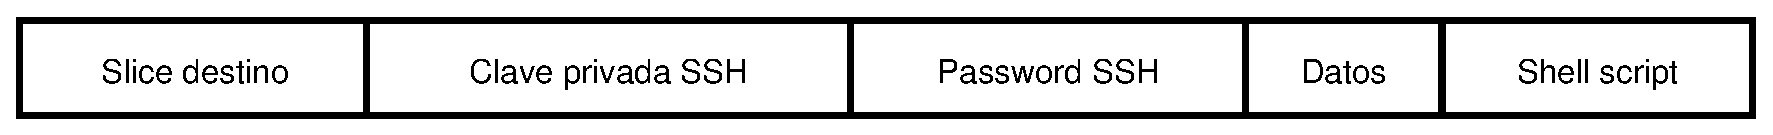
\includegraphics[scale=0.5]{paq_-_uplfs-pldb.eps}
	\caption{Paquete generico \uplfs $\rightarrow$ \dplc}
	\label{fig:paq_-_uplfs-pldb}
\end{figure}


\subsubsection{Datos}
% TODO: En caso de que el paquete contenga el campo \texttt{Cmd}.....

\begin{figure}[h]
	\centering
	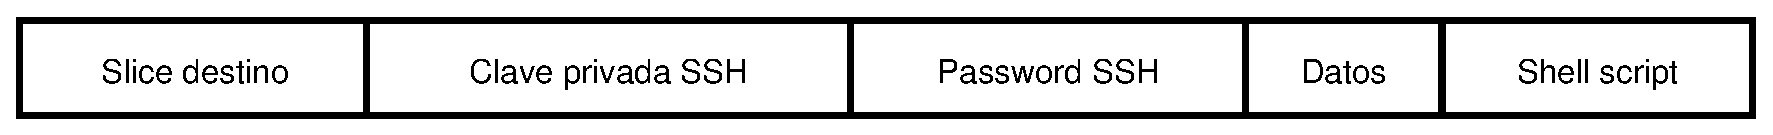
\includegraphics[scale=0.5]{paq_-_uplfs-pldb_-_data.eps}
	\caption{Paquete de datos \uplfs $\rightarrow$ \dplc}
	\label{fig:paq_-_uplfs-pldb_-_data}
\end{figure}

% TODO: Datos => lista ficheros + ficheros?
%       (kernel permite agrupaci�n de ficheros en un env�o?)
% TODO: si ya se pre-acredita, no hace falta ahora enviar passwd+clave
% TODO: otros tipos de paquete?

\begin{description}
	\item[Slice destino:] nombre del slice destino al que va destinado el
		paquete

	\item[Clave/Passwordd privados ssh:] clave y password privados de ssh para
		que	\dplc se comunique con el slice destino

	\item[Datos:] datos a desplegar en el slice destino

	\item[Shell script:] shell script a ejecutar una vez desplegados los
		ficheros (optativo)
\end{description}


\subsubsection{Registro de oyente}

% TODO Formate de paquete de registro



\section{\dplc $\rightarrow$ \dpld}

Los nodos \dplc deben informar de los cambios en los grupos slice destino
a los \dpld que est�n registrados en ellos para esos slice.

Los cambios pueden ser:
\begin{itemize}
	\item Se a�ade un nuevo nodo al slice.

	\item Se quita un nodo del slice.

	\item Modificaci�n de ficheros (invalidaci�n).
\end{itemize}

Para anunciar estos cambios hemos dise�ado un paquete de warning mediante el
cual los nodos \dplc los anuncian a los \dpld registrados.

%TODO figura paquete warning
Campo 1: tipo de cambio.
Campo 2: string (nodo o fichero).
Campo 3: shared o unshared
...

Para autentificar los paquetes de warning se firman con la clave privada
de \dplc.

